\documentclass{article}
\usepackage[a4paper]{geometry}
\usepackage[skip=10pt]{parskip}
\usepackage{amssymb}
\usepackage{graphicx}
\usepackage{hyperref}
\usepackage[section]{placeins}
\usepackage[official]{eurosym}
\usepackage{textgreek}
\usepackage{tcolorbox}
\usepackage{listings}
\usepackage{textcomp}
\usepackage{ccicons}
\usepackage{tikz}

\renewcommand{\familydefault}{\sfdefault}

\setlength\parindent{0pt}

\newenvironment{note}{\begin{tcolorbox}[colback=blue!5!white,colframe=blue!75!black,title=\textbf{Note}]}{\end{tcolorbox}}
\newenvironment{caution}{\begin{tcolorbox}[colback=red!5!white,colframe=red!75!black,title=\textbf{Caution}]}{\end{tcolorbox}}
\newcommand{\file}[1]{\texttt{#1}}

\lstset
{
	basicstyle=\footnotesize\ttfamily,
	breaklines=true,
	keywordstyle=\bfseries\color{green!40!black},
	commentstyle=\itshape\color{purple!40!black},
	identifierstyle=\color{blue},
	stringstyle=\color{orange},
	tabsize=4
}

\begin{document}
\hypersetup{pageanchor=false}
\begin{titlepage}
\thispagestyle{empty}
\centering
\textsf{\Huge MacroPad}\\[1cm]
\textsf{\Large Programmable USB Input Device}\\[3cm]
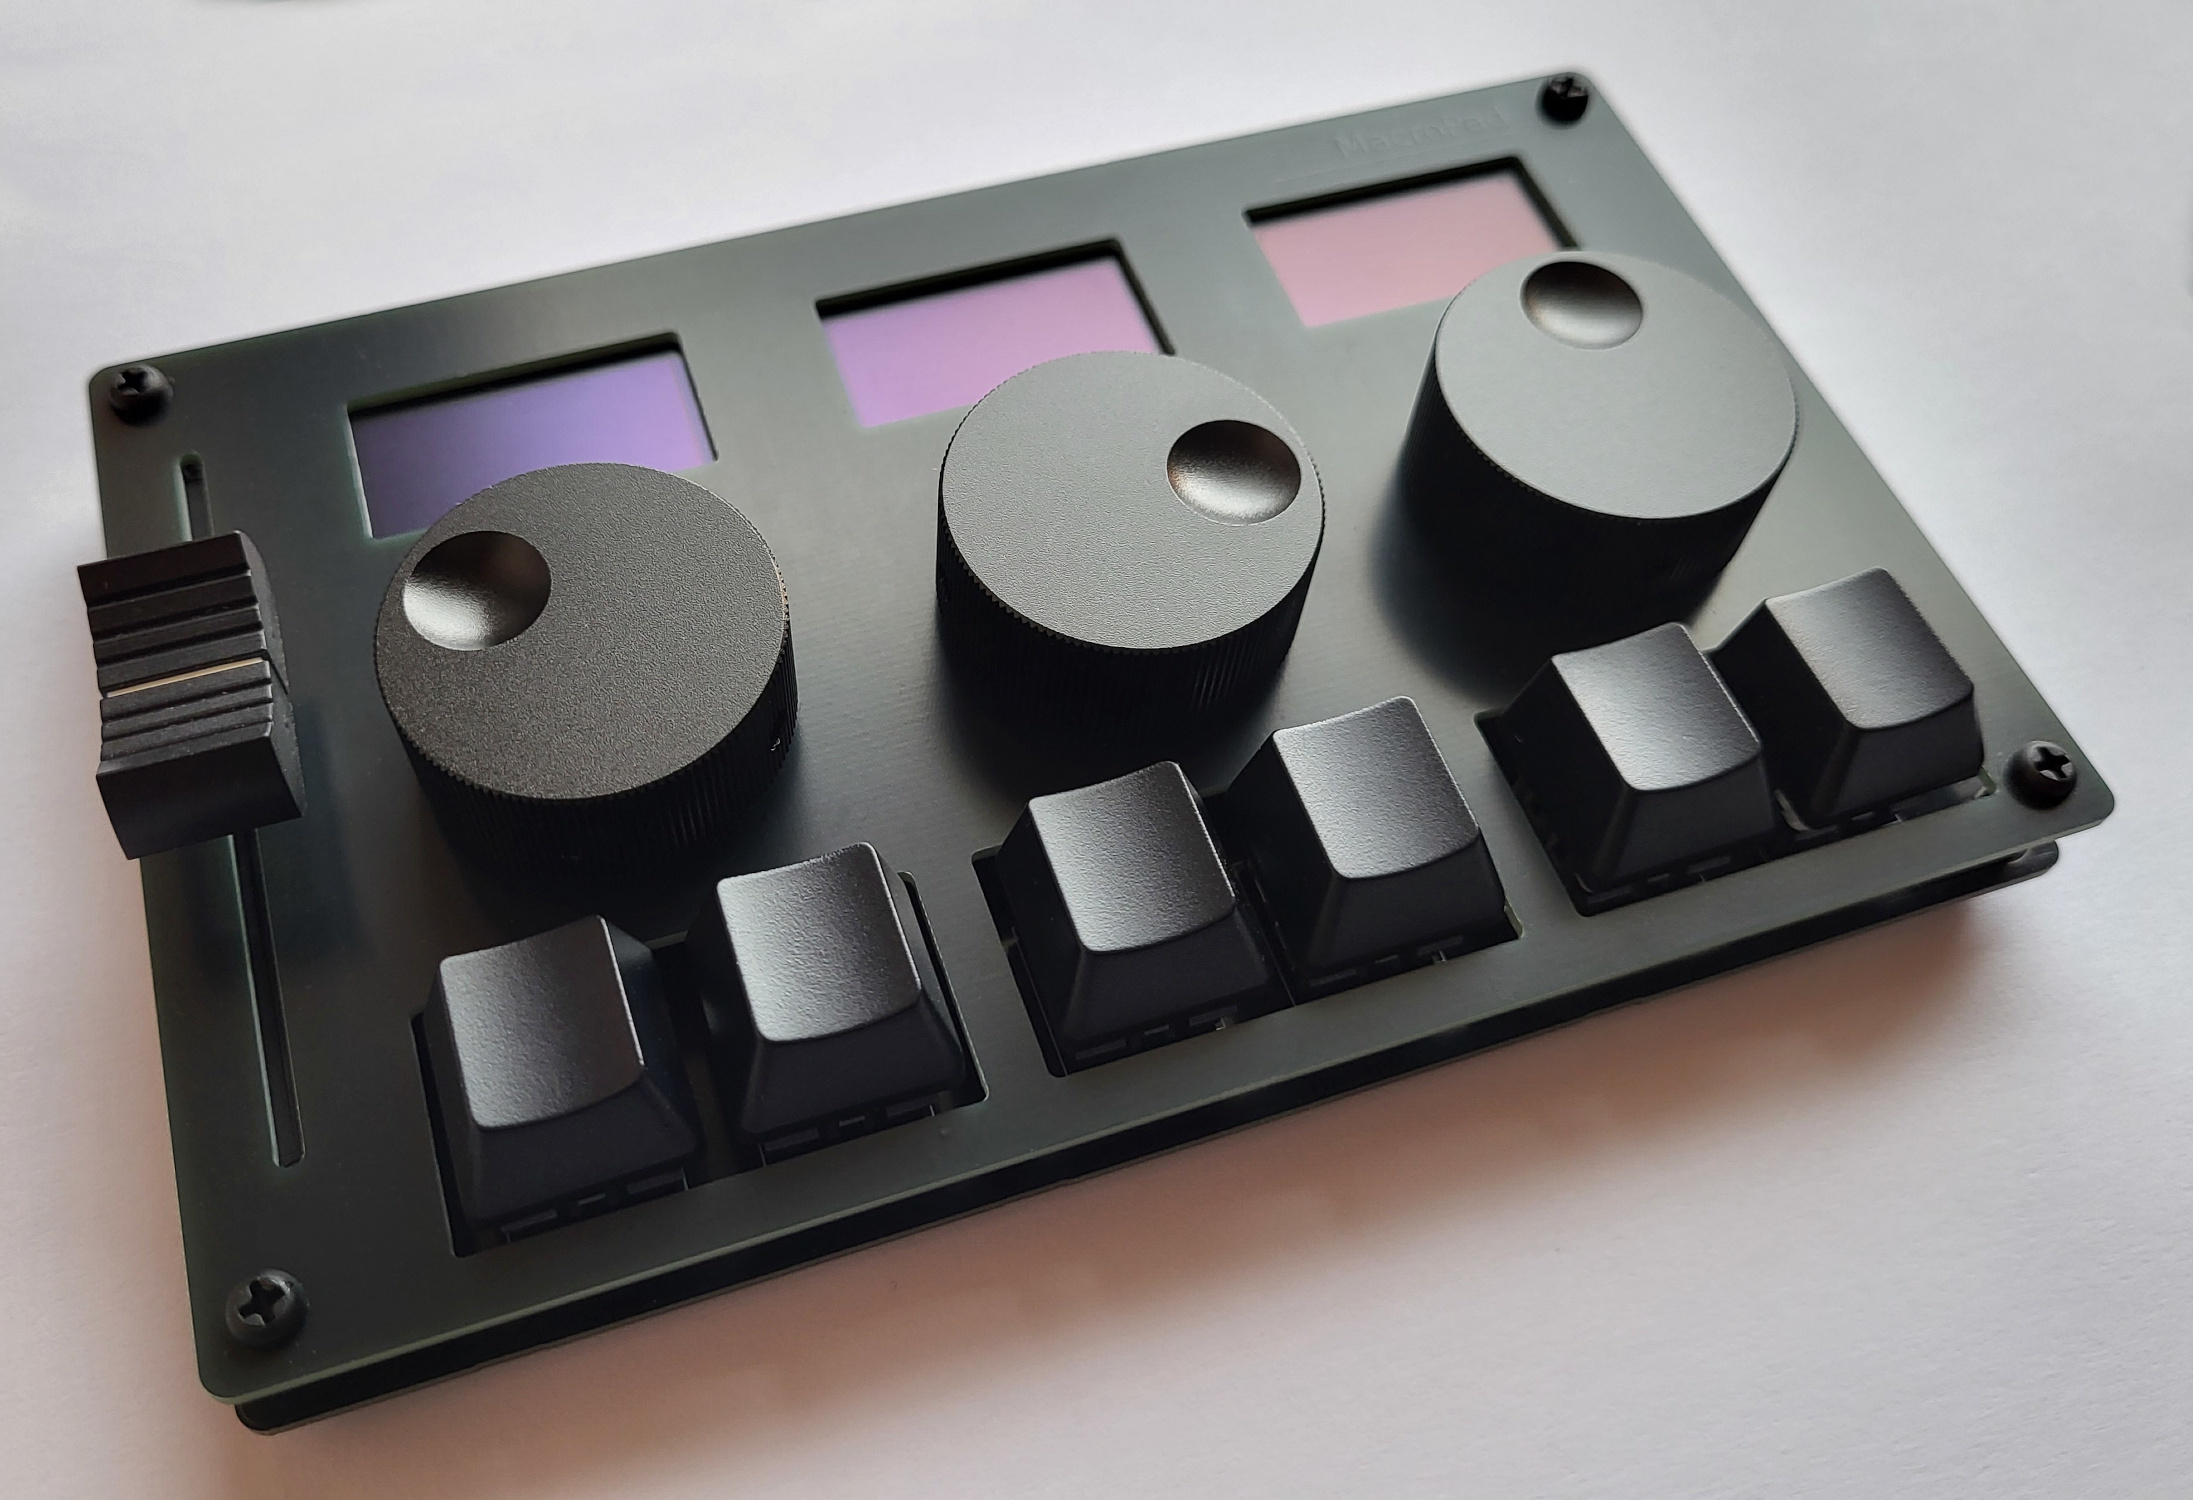
\includegraphics[width=\textwidth]{Images/Title.jpg}\\[3cm]
\textsf{\Large User's Guide}
\end{titlepage}
\hypersetup{pageanchor=true}

\section*{License}
This document is licensed under Creative Commons \href{https://creativecommons.org/licenses/by-nc/4.0/}{Attribution-NonCommercial 4.0 International} (CC BY-NC 4.0 \ccCopy\,\ccAttribution\,\ccNonCommercial).

Attribution to \href{http://github.com/7vgn/MacroPad/}{http://github.com/7vgn/MacroPad/} is sufficient.
\tableofcontents

\section{Introduction}
MacroPad is a USB input device with three knobs, one slider, and six keys. It also features three OLED displays to show the current bindings of the input controls. Figure \ref{fig:overview} shows the positions of all the controls.
\begin{figure}[htb]
\centering
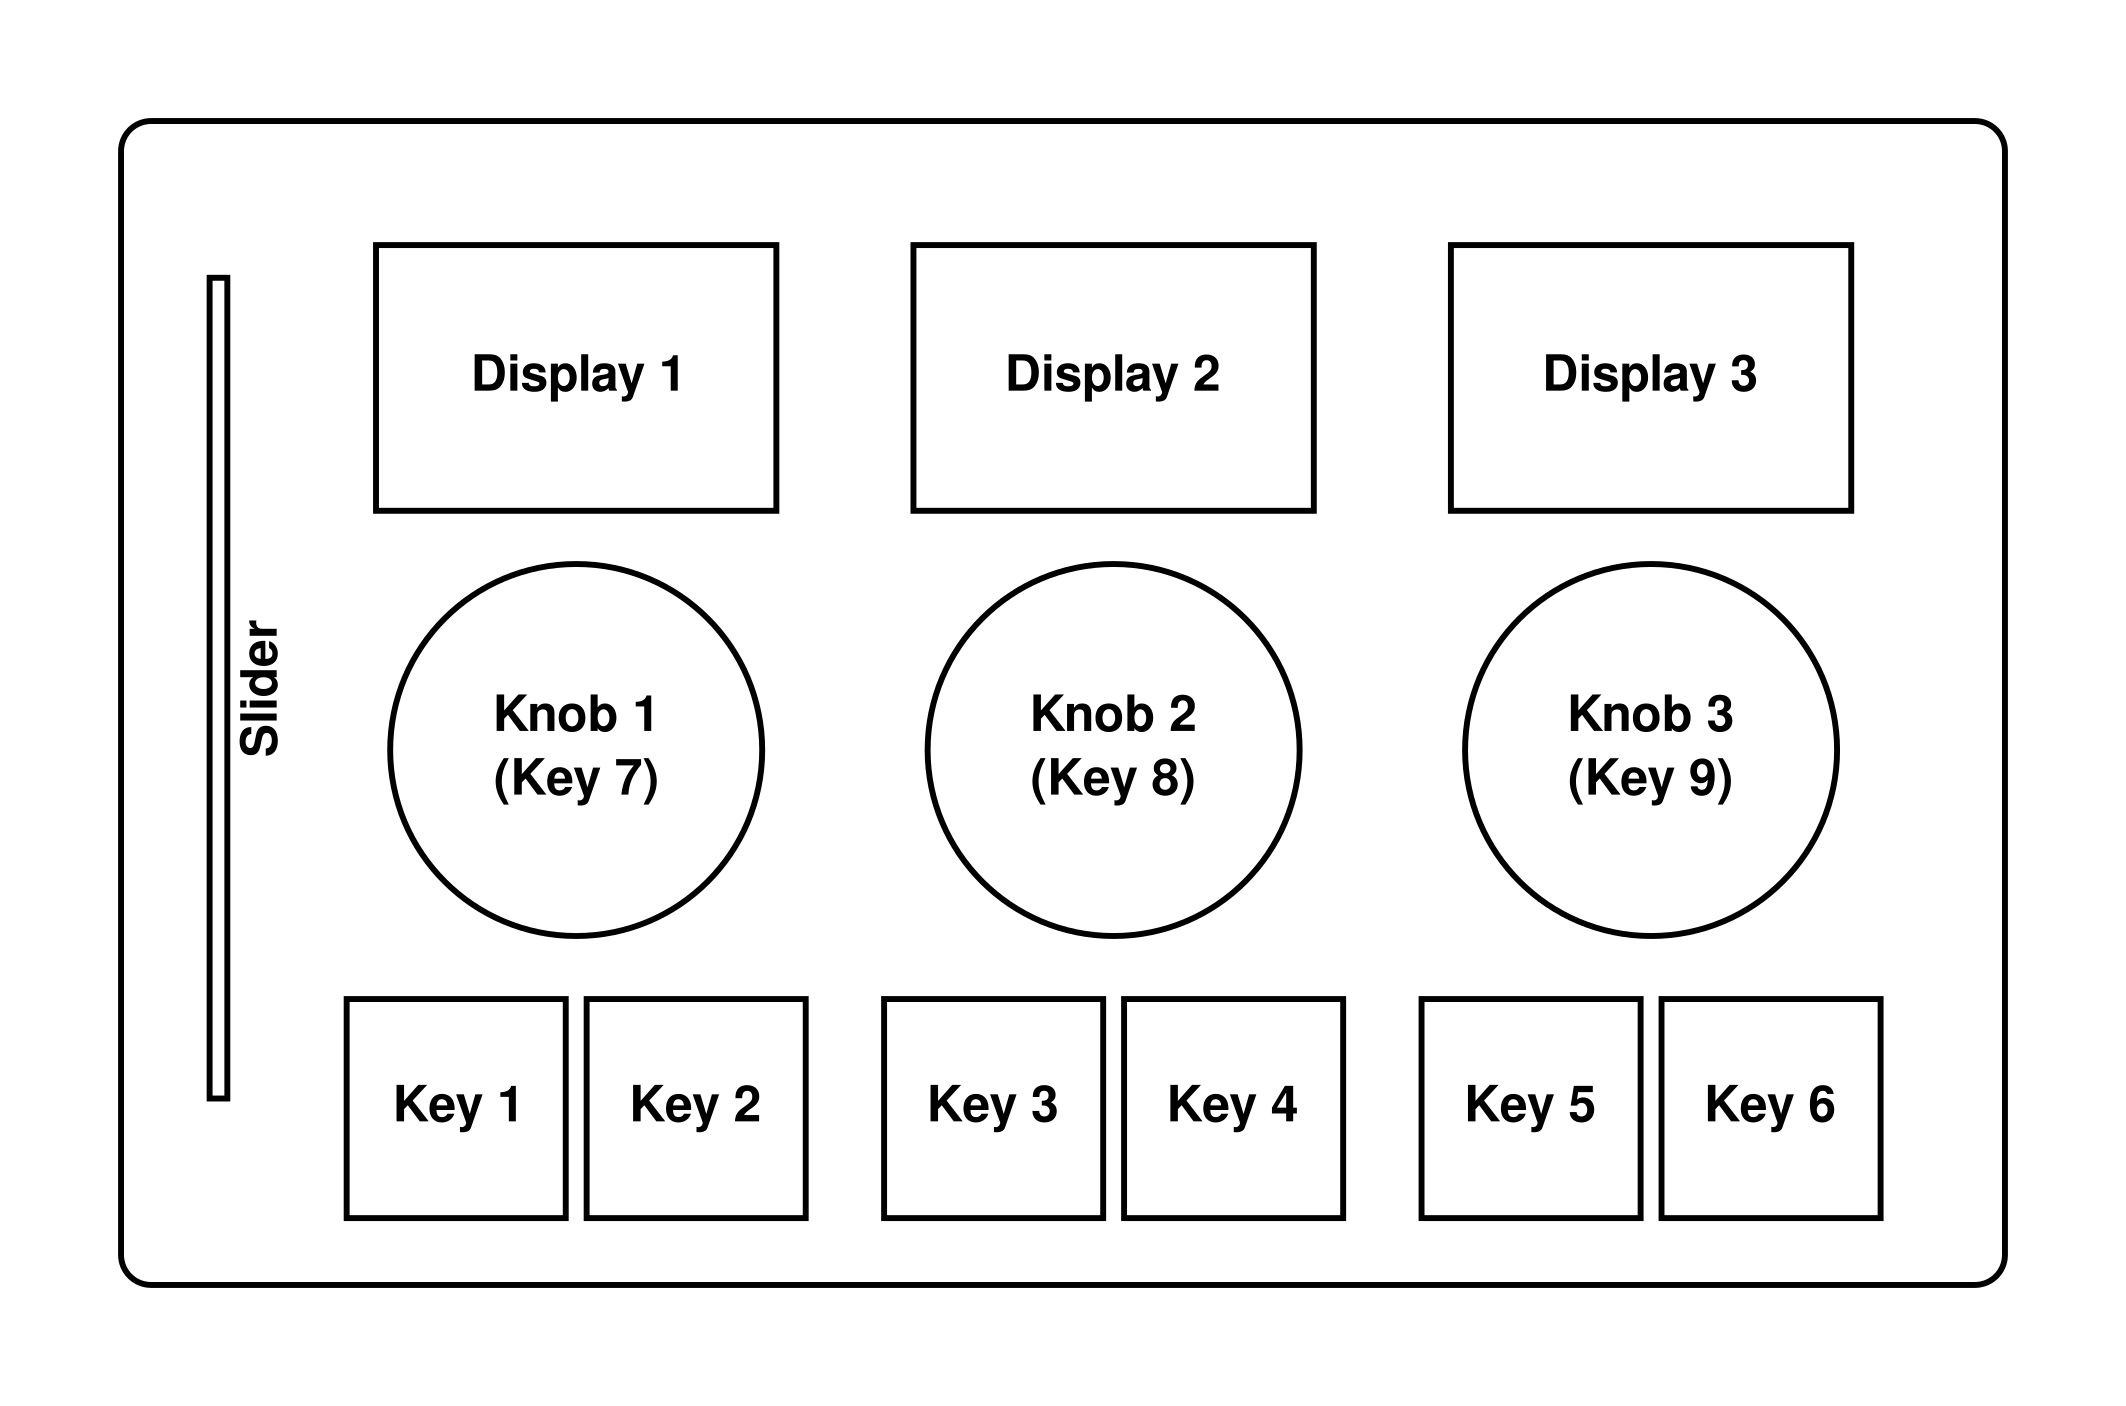
\includegraphics[width=\textwidth]{Images/Overview.png}
\caption{Overview of the Device}
\label{fig:overview}
\end{figure}

The knobs can not just be turned but also pressed which is why they are also listed as keys.

During normal operation, Display 1 will show the bindings of the input controls below it, that is Keys 1 and 2, as well as Knob 1 (including Key 7). The same goes for the other two displays.

MacroPad presents itself to the computer as a combination of standard USB input devices (a keyboard, a mouse etc.). This means it should work on any operating system without the need for a driver.\\
Additional software might be required if you want it to perform actions that go beyond what keyboard/mouse/etc.\ inputs can do (for example performing actions in specific applications that don't have hotkeys).

\section{Customise MacroPad}\label{sec:customise}
\subsection{How Settings Work: Actions, Macros, and Profiles}\label{sec:settings}
MacroPad supports multiple profiles that you can switch between. The active profile defines what is sent to the computer in reaction to the user interacting with the input controls. Profiles also define the images shown on the displays and a few other things.

Having multiple profiles allows you to reconfigure MacroPad quickly without having to upload new settings. For example, you might want to create different profiles for different applications, although they are not necessarily tied to that. You might have multiple profiles for the same application or simple just one profile for everything.

To understand how a profile maps user inputs to signals sent over USB, we need to define some terms:

An \emph{Action} is a piece of information (e.g.\ ``ctrl key and right mouse button are pressed'') sent to the host over USB. Being a USB HID\footnote{Human Interface Device}-class device, MacroPad sends a report every 10 milliseconds. Such a report contains a list of all the keys and mouse buttons that are currently down, as well as incremental changes (e.g.\ how far has the mouse moved in x direction since the last report). MacroPad combines all current actions (from the different input controls) into a report which it then sends to the host.

A \emph{Macro} is a sequence of actions, with a duration for each action. A macro might for example look like this: Have the left mouse button and the shift key down (first action) for 20ms. Then move the mouse downwards at a rate of five units per 10ms (second action) for 30ms. After that, have the alt and enter keys down (third action) for 10ms.
Executing this macro would take 60ms during which time seven reports would be sent (the seventh report being ``all keys have been released'').

There are two types of user input events: First, we have keys being held down, i.e.\ events that occur over a period of time. Such an event causes an action to be continuously reported as long as the key is down.
The second type of event concerns singular points in time: This includes button presses and releases, as well as rotating a knob one notch to the left or right. These kinds of events trigger macros.

There is no dedicated key for switching between profiles. Instead, profile switching is just a special kind of action. This means you can assign it freely to any key or knob event in each profile. Or not -- if you're only using a single profile -- thus gaining more space for other actions.

\subsection{The MacroPad Settings App}\label{sec:settings_app}
MacroPad comes with an graphical user interface app that allows you to create, modify, and upload settings. You can also store settings in an XML file on your computer.

The Settings App is called \lstinline[language=bash]{MacroPad} (\lstinline[language=bash]{MacroPad.exe} on Windows). There is no installer -- just copy the executable file to some place on your computer and run it.

The Settings App should be pretty self-explanatory. Each profile is configured in a separate tab. In order to change the behaviour of an input control (like a key), click on it, then edit the macro or action. You can create or import custom pictures for each profile, key, and knob.
If you're using multiple profiles, don't forget to configure one of the input controls to switch between them.

If you're overwhelmed by the options, you can load and modify an existing settings file instead.

Once you have created your personalised settings, it is recommended that you save them in a file for safekeeping.
In order to write them to the device, hit the ``Scan for Devices'' button, choose the correct MacroPad device from the drop-down (in case you have multiple), then hit ``Write to Device''. After a few seconds, your MacroPad should have its new settings.
\begin{note}
Do not unplug the device while settings are transferred.
\end{note}

\subsubsection{User priviledges on Linux}\label{sec:linux_priviledges}
On Linux, the app must be run with root proviledges (``sudo'') since normal users are not allowed to access USB devices.

If you don't want that, you can add an exception for MacroPad: The following steps describe how to do this on Debian-based distributions like Ubuntu. On other Linux systems there might be slight differences.
\begin{enumerate}
\item Open a terminal and run \lstinline[language=bash]{lsusb}.
If lsusb is not on your system you can get it by installing the usbutils package:
\begin{lstlisting}[language=bash]
sudo apt-get install usbutils
\end{lstlisting}
Find the line with the MacroPad device and note down the Vendor ID (VID) and Product ID (PID). These are 4-letter/digit codes separated by a colon (VID:PID).\\
\item In a text editor of your choice, create a file named ``69-MacroPad.rules'' with the following content:\\
~\\
\texttt{SUBSYSTEMS=="usb", ATTRS{idVendor}=="VID", ATTRS{idProduct}=="PID", TAG+="uaccess"
KERNEL=="hidraw", ATTRS{idVendor}=="VID", ATTRS{idProduct}=="PID", TAG+="uaccess"}
~\\
Replace ``VID'' and ``PID'' with the IDs noted down before.
\item Copy the file to /etc/udev/rules.d/ (you must use root priviledges to do that):
\begin{lstlisting}[language=bash]
sudo cp 69-MacroPad.rules /etc/udev/rules.d/.
\end{lstlisting}
\item Restart your computer or run the following commands:
\begin{lstlisting}[language=bash]
sudo udevadm control --reload-rules
sudo udevadm trigger
\end{lstlisting}
\end{enumerate}

\subsection{The Command Line Settings Tool}\label{sec:cmdline_tool}
There is a command line-based alternative for the Settings App, called \lstinline[language=bash]{macropad-cli}. It can transfer the same XML settings files from and to MacroPad devices as the graphical Settings App. For more information on how to use the command-line tool, run:
\begin{lstlisting}[language=bash]
macropad-cli --help
\end{lstlisting}
The command-line tool provides no means for creating and editing settings files. For this, you need either the graphical Settings App or edit the XML file by hand.
Unless you have a very particular use case, we recommend you use the graphical Settings App instead.

\section{Firmware Update}\label{sec:firmwareupdate}
\begin{note}
Sections \ref{sec:flash} and \ref{sec:restoresettings} also apply to the initial flashing of the firmware onto an empty device.
\end{note}

\subsection{Save Your Settings}\label{sec:savesettings}
Firmware updates do not preserve the settings. If you want to keep your profiles, read them from the device and store them in a file on your computer before starting the firmware update process. See Section \ref{sec:settings_app} for details.
Make sure to use the old Settings App to do this. The Settings App can only read settings from a device with the same firmware version.

\subsection{Flash the New Firmware}\label{sec:flash}
Download the new firmware. It comes in a file ending in ``.uf2''.
\begin{enumerate}
\item Unplug your device.
\item Locate the ``BOOTSEL'' button. The labels on the back of device can help you find it.
\item Press the button and keep holding it, while plugging the USB cable from your computer into the device.
\item Your computer should recognize it as a mass storage device. On most operating systems, a file manager window will pop up.
\item Release the button.
\item Copy the new firmware file onto the device.
\item The mass storage device will immediately self-eject and MacroPad reappears as several input devices. If it doesn't, unplug and replug the USB cable.
\end{enumerate}

\subsection{Restore Your Settings}\label{sec:restoresettings}
Now you can write your settings back onto the device as described in Section \ref{sec:settings_app}.
Make sure to use the new Settings App to do this. The Settings App can only write settings to a device with the same firmware version.

\end{document}
